% !Mode:: "TeX::UTF-8"

\documentclass[oneside]{book}

%========基本必备的宏包========%
\usepackage[a4paper,
  bindingoffset=10mm,%裝訂線
  top=35mm,  %上邊距 包括頁眉
  bottom=30mm,%下邊距 包括頁腳
  inner=10mm,  %左邊距or inner
  outer=10mm,  %右邊距or  outer
  headheight=10mm,%頁眉
  headsep=15mm,%
  footskip=15mm,%
  marginparsep=0pt, %旁註與正文間距
  marginparwidth=0em,includemp=true% 旁註寬度計入width%旁註寬度
  symmetric 
  ]{geometry}

\usepackage[UTF8, heading=true, scheme=chinese, fontset=none]{ctex}
\ctexset{fontset = fandol}

\usepackage{microtype} % 提高排版质量
\usepackage{setspace} % 设置行间距
\usepackage{hyperref}
\usepackage{xcolor}  % 颜色支持
\usepackage{xpinyin} % 拼音宏包
\usepackage{tikz}    % 用于绘制删除线
\usepackage{array}

% 定义一个新的删除线命令,使用tikz绘制
\newcommand{\strike}[1]{%
  \tikz[baseline=(text.base)]{
    \node[inner sep=0pt, outer sep=0pt] (text) {#1};
    \draw[red, line width=3pt] (text.south west) -- (text.north east);
  }%
}

\newcommand{\largefont}{\fontsize{28pt}{34pt}\selectfont}



\hypersetup{
    colorlinks=true,
    linkcolor=blue,
    citecolor=green,
    filecolor=magenta,
    urlcolor=cyan
}

\title{拼音表}
\author{田利建}
\date{\today}

\begin{document}

\maketitle


\section{b、p、m、f}

\begin{center}
\renewcommand{\arraystretch}{3} % 增加行间距
\xpinyinsetup{ % 调整拼音字体大小
  font={\fontspec{DejaVu Sans Mono}\fontsize{36pt}{40pt}\selectfont},
}
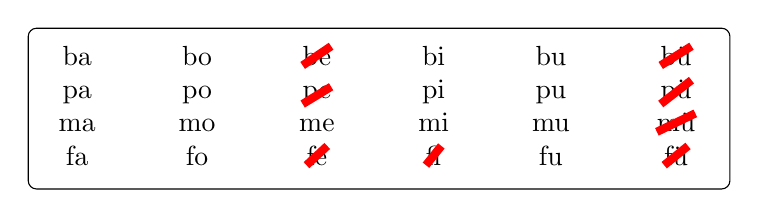
\begin{tikzpicture}
\node[draw, inner sep=5pt, rounded corners=3pt] {
\begin{tabular}{c@{\hspace{3em}}c@{\hspace{3em}}c@{\hspace{3em}}c@{\hspace{3em}}c@{\hspace{3em}}c}
  \pinyin{ba} & \pinyin{bo} & \strike{\pinyin{be}} & \pinyin{bi} & \pinyin{bu} & \strike{\pinyin{bü}} \\
  \pinyin{pa} & \pinyin{po} & \strike{\pinyin{pe}} & \pinyin{pi} & \pinyin{pu} & \strike{\pinyin{pü}} \\
  \pinyin{ma} & \pinyin{mo} & \pinyin{me} & \pinyin{mi} & \pinyin{mu} & \strike{\pinyin{mü}} \\
  \pinyin{fa} & \pinyin{fo} & \strike{\pinyin{fe}} & \strike{\pinyin{fi}} & \pinyin{fu} & \strike{\pinyin{fü}} \\
\end{tabular}
};
\end{tikzpicture}

\vspace{5em}

\renewcommand{\arraystretch}{5} % 增加行间距
\xpinyinsetup{ % 调整拼音字体大小
  font={\fontspec{DejaVu Sans Mono}\selectfont},
  ratio={1},
  hsep={.5em plus .3em minus .3em},
  vsep={1em}
}
\begin{tikzpicture}
\node[draw, inner sep=5pt, rounded corners=3pt] {
\begin{tabular}{>{\largefont}c@{\hspace{3em}}>{\largefont}c@{\hspace{3em}}>{\largefont}c@{\hspace{3em}}>{\largefont}c@{\hspace{3em}}>{\largefont}c@{\hspace{3em}}>{\largefont}c@{\hspace{3em}}}
  \xpinyin{八}{ba} & \xpinyin{波}{bo} & \strike{\pinyin{be}} & \xpinyin{比}{bi} & \xpinyin{不}{bu} & \strike{\pinyin{bü}} \\  % 汉字无需加命令
  \xpinyin{怕}{pa} & \xpinyin{破}{po} & \strike{\pinyin{pe}} & \xpinyin{皮}{pi} & \xpinyin{普}{pu} & \strike{\pinyin{pü}} \\
  \xpinyin{妈}{ma} & \xpinyin{陌}{mo} & \xpinyin{么}{me} & \xpinyin{米}{mi} & \xpinyin{木}{mu} & \strike{\pinyin{mü}} \\
  \xpinyin{发}{fa} & \xpinyin{佛}{fo} & \strike{\pinyin{fe}} & \strike{\pinyin{fi}} & \xpinyin{夫}{fu} & \strike{\pinyin{fü}} \\
\end{tabular}
};
\end{tikzpicture}
\end{center}

\section{d、t、n、l}

\begin{center}
\renewcommand{\arraystretch}{3} % 增加行间距
\xpinyinsetup{ % 调整拼音字体大小
  font={\fontspec{DejaVu Sans Mono}\fontsize{36pt}{40pt}\selectfont},
}
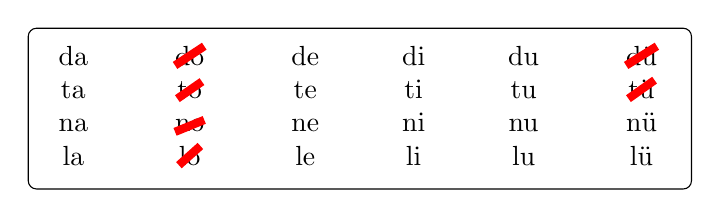
\begin{tikzpicture}
\node[draw, inner sep=5pt, rounded corners=3pt] {
\begin{tabular}{c@{\hspace{3em}}c@{\hspace{3em}}c@{\hspace{3em}}c@{\hspace{3em}}c@{\hspace{3em}}c}
  \pinyin{da} & \strike{\pinyin{do}} & \pinyin{de} & \pinyin{di} & \pinyin{du} & \strike{\pinyin{dü}} \\
  \pinyin{ta} & \strike{\pinyin{to}} & \pinyin{te} & \pinyin{ti} & \pinyin{tu} & \strike{\pinyin{tü}} \\
  \pinyin{na} & \strike{\pinyin{no}} & \pinyin{ne} & \pinyin{ni} & \pinyin{nu} & \pinyin{nü} \\
  \pinyin{la} & \strike{\pinyin{lo}} & \pinyin{le} & \pinyin{li} & \pinyin{lu} & \pinyin{lü} \\
\end{tabular}
};
\end{tikzpicture}

\vspace{2em}

\renewcommand{\arraystretch}{5} % 增加行间距
\xpinyinsetup{ % 调整拼音字体大小
  font={\fontspec{DejaVu Sans Mono}\selectfont},
  ratio={1},
  hsep={.5em plus .3em minus .3em},
  vsep={1em}
}
\begin{tikzpicture}
\node[draw, inner sep=5pt, rounded corners=3pt] {
\begin{tabular}{>{\largefont}c@{\hspace{3em}}>{\largefont}c@{\hspace{3em}}>{\largefont}c@{\hspace{3em}}>{\largefont}c@{\hspace{3em}}>{\largefont}c@{\hspace{3em}}>{\largefont}c@{\hspace{3em}}}
  \xpinyin{大}{da} & \strike{\pinyin{do}} & \xpinyin{的}{de} & \xpinyin{地}{di} & \xpinyin{读}{du} & \strike{\pinyin{dü}} \\
  \xpinyin{他}{ta} & \strike{\pinyin{to}} & \xpinyin{特}{te} & \xpinyin{体}{ti} & \xpinyin{土}{tu} & \strike{\pinyin{tü}} \\
  \xpinyin{那}{na} & \strike{\pinyin{no}} & \xpinyin{呢}{ne} & \xpinyin{你}{ni} & \xpinyin{努}{nu} & \xpinyin{女}{nü} \\
  \xpinyin{拉}{la} & \strike{\pinyin{lo}} & \xpinyin{乐}{le} & \xpinyin{利}{li} & \xpinyin{路}{lu} & \xpinyin{旅}{lü} \\
\end{tabular}
};
\end{tikzpicture}
\end{center}

\section{g、k、h}

\begin{center}
\renewcommand{\arraystretch}{3} % 增加行间距
\xpinyinsetup{ % 调整拼音字体大小
  font={\fontspec{DejaVu Sans Mono}\fontsize{36pt}{40pt}\selectfont},
}
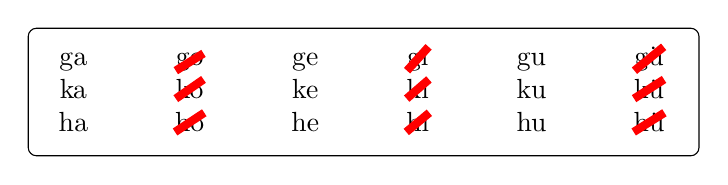
\begin{tikzpicture}
\node[draw, inner sep=5pt, rounded corners=3pt] {
\begin{tabular}{c@{\hspace{3em}}c@{\hspace{3em}}c@{\hspace{3em}}c@{\hspace{3em}}c@{\hspace{3em}}c}
  \pinyin{ga} & \strike{\pinyin{go}} & \pinyin{ge} & \strike{\pinyin{gi}} & \pinyin{gu} & \strike{\pinyin{gü}} \\
  \pinyin{ka} & \strike{\pinyin{ko}} & \pinyin{ke} & \strike{\pinyin{ki}} & \pinyin{ku} & \strike{\pinyin{kü}} \\
  \pinyin{ha} & \strike{\pinyin{ho}} & \pinyin{he} & \strike{\pinyin{hi}} & \pinyin{hu} & \strike{\pinyin{hü}} \\
\end{tabular}
};
\end{tikzpicture}

\vspace{2em}

\renewcommand{\arraystretch}{5} % 增加行间距
\xpinyinsetup{ % 调整拼音字体大小
  font={\fontspec{DejaVu Sans Mono}\selectfont},
  ratio={1},
  hsep={.5em plus .3em minus .3em},
  vsep={1em}
}
\begin{tikzpicture}
\node[draw, inner sep=5pt, rounded corners=3pt] {
\begin{tabular}{>{\largefont}c@{\hspace{3em}}>{\largefont}c@{\hspace{3em}}>{\largefont}c@{\hspace{3em}}>{\largefont}c@{\hspace{3em}}>{\largefont}c@{\hspace{3em}}>{\largefont}c@{\hspace{3em}}}
  \xpinyin{嘎}{ga} & \strike{\pinyin{go}} & \xpinyin{个}{ge} & \strike{\pinyin{gi}} & \xpinyin{古}{gu} & \strike{\pinyin{gü}} \\
  \xpinyin{卡}{ka} & \strike{\pinyin{ko}} & \xpinyin{可}{ke} & \strike{\pinyin{ki}} & \xpinyin{苦}{ku} & \strike{\pinyin{kü}} \\
  \xpinyin{哈}{ha} & \strike{\pinyin{ho}} & \xpinyin{和}{he} & \strike{\pinyin{hi}} & \xpinyin{胡}{hu} & \strike{\pinyin{hü}} \\
\end{tabular}
};
\end{tikzpicture}
\end{center}

\end{document}
